\documentclass[]{article}
\usepackage{lmodern}
\usepackage{amssymb,amsmath}
\usepackage{ifxetex,ifluatex}
\usepackage{fixltx2e} % provides \textsubscript
\ifnum 0\ifxetex 1\fi\ifluatex 1\fi=0 % if pdftex
  \usepackage[T1]{fontenc}
  \usepackage[utf8]{inputenc}
\else % if luatex or xelatex
  \ifxetex
    \usepackage{mathspec}
  \else
    \usepackage{fontspec}
  \fi
  \defaultfontfeatures{Ligatures=TeX,Scale=MatchLowercase}
\fi
% use upquote if available, for straight quotes in verbatim environments
\IfFileExists{upquote.sty}{\usepackage{upquote}}{}
% use microtype if available
\IfFileExists{microtype.sty}{%
\usepackage{microtype}
\UseMicrotypeSet[protrusion]{basicmath} % disable protrusion for tt fonts
}{}
\usepackage[margin=1in]{geometry}
\usepackage{hyperref}
\hypersetup{unicode=true,
            pdfborder={0 0 0},
            breaklinks=true}
\urlstyle{same}  % don't use monospace font for urls
\usepackage{graphicx,grffile}
\makeatletter
\def\maxwidth{\ifdim\Gin@nat@width>\linewidth\linewidth\else\Gin@nat@width\fi}
\def\maxheight{\ifdim\Gin@nat@height>\textheight\textheight\else\Gin@nat@height\fi}
\makeatother
% Scale images if necessary, so that they will not overflow the page
% margins by default, and it is still possible to overwrite the defaults
% using explicit options in \includegraphics[width, height, ...]{}
\setkeys{Gin}{width=\maxwidth,height=\maxheight,keepaspectratio}
\IfFileExists{parskip.sty}{%
\usepackage{parskip}
}{% else
\setlength{\parindent}{0pt}
\setlength{\parskip}{6pt plus 2pt minus 1pt}
}
\setlength{\emergencystretch}{3em}  % prevent overfull lines
\providecommand{\tightlist}{%
  \setlength{\itemsep}{0pt}\setlength{\parskip}{0pt}}
\setcounter{secnumdepth}{0}
% Redefines (sub)paragraphs to behave more like sections
\ifx\paragraph\undefined\else
\let\oldparagraph\paragraph
\renewcommand{\paragraph}[1]{\oldparagraph{#1}\mbox{}}
\fi
\ifx\subparagraph\undefined\else
\let\oldsubparagraph\subparagraph
\renewcommand{\subparagraph}[1]{\oldsubparagraph{#1}\mbox{}}
\fi

%%% Use protect on footnotes to avoid problems with footnotes in titles
\let\rmarkdownfootnote\footnote%
\def\footnote{\protect\rmarkdownfootnote}

%%% Change title format to be more compact
\usepackage{titling}

% Create subtitle command for use in maketitle
\newcommand{\subtitle}[1]{
  \posttitle{
    \begin{center}\large#1\end{center}
    }
}

\setlength{\droptitle}{-2em}

  \title{}
    \pretitle{\vspace{\droptitle}}
  \posttitle{}
    \author{}
    \preauthor{}\postauthor{}
    \date{}
    \predate{}\postdate{}
  

\begin{document}

\hypertarget{regional-stats-plot-gallery}{%
\section{Regional Stats Plot
Gallery}\label{regional-stats-plot-gallery}}

\hypertarget{comparison-barplots}{%
\subsubsection{comparison barplots}\label{comparison-barplots}}

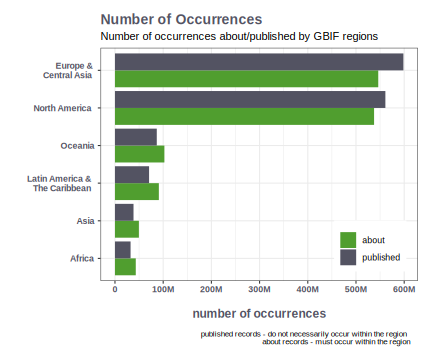
\includegraphics{C:/Users/ftw712/Desktop/gbif_regional_statistics/plots/comparison barchart/svg/gbif_regions_occ_count.svg}

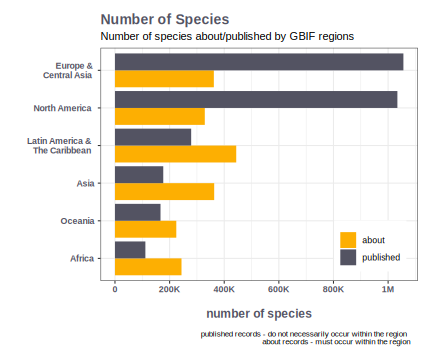
\includegraphics{C:/Users/ftw712/Desktop/gbif_regional_statistics/plots/comparison barchart/svg/gbif_regions_num_species.svg}

\hypertarget{hexagon-plots}{%
\subsubsection{Hexagon Plots}\label{hexagon-plots}}

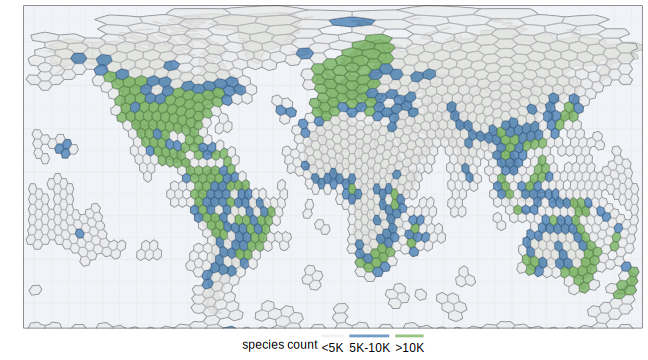
\includegraphics{C:/Users/ftw712/Desktop/gbif_regional_statistics/plots/hexagon plots/global_num_species.jpg}

\includegraphics{C:/Users/ftw712/Desktop/gbif_regional_statistics/plots/hexagon plots/afrca_num_species.jpg}

\hypertarget{time-series-snapshot-plots}{%
\subsubsection{Time series snapshot
plots}\label{time-series-snapshot-plots}}

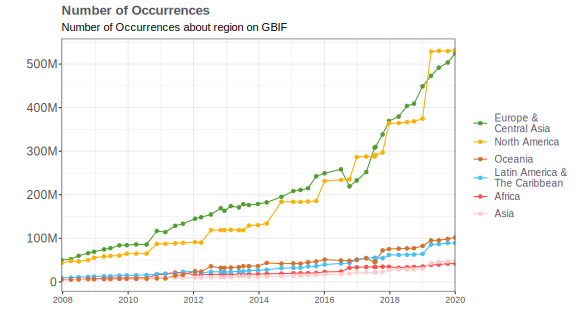
\includegraphics{C:/Users/ftw712/Desktop/gbif_regional_statistics/plots/time series/timeseries_num_occ.svg}

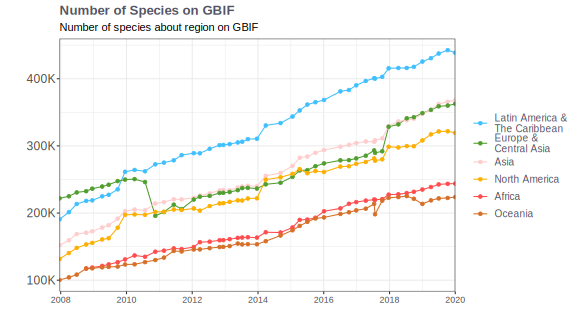
\includegraphics{C:/Users/ftw712/Desktop/gbif_regional_statistics/plots/time series/timeseries_num_species.svg}

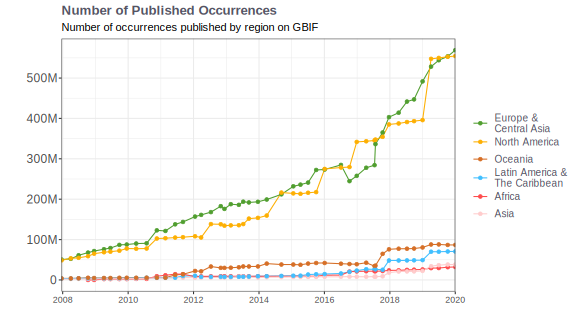
\includegraphics{C:/Users/ftw712/Desktop/gbif_regional_statistics/plots/time series/timeseries_num_occ_published.svg}

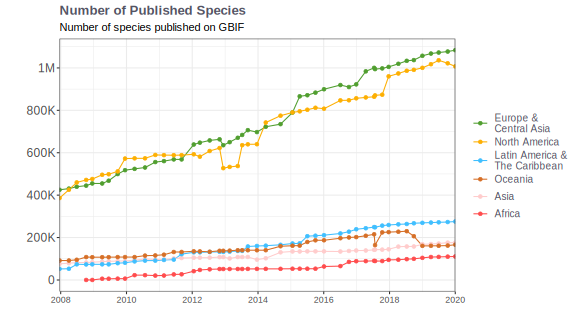
\includegraphics{C:/Users/ftw712/Desktop/gbif_regional_statistics/plots/time series/timeseries_num_species_published.svg}

\hypertarget{dotplots}{%
\subsubsection{Dotplots}\label{dotplots}}

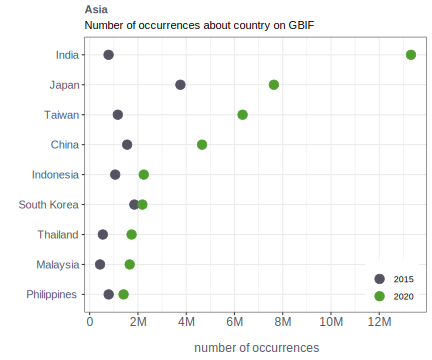
\includegraphics{C:/Users/ftw712/Desktop/gbif_regional_statistics/plots/country dotplots/country_dotplot_occ_count_Asia.svg}

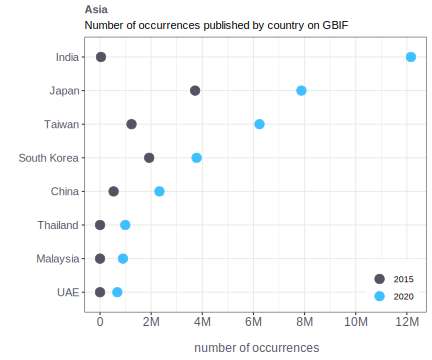
\includegraphics{C:/Users/ftw712/Desktop/gbif_regional_statistics/plots/country dotplots/country_dotplot_occ_count_published_Asia.svg}

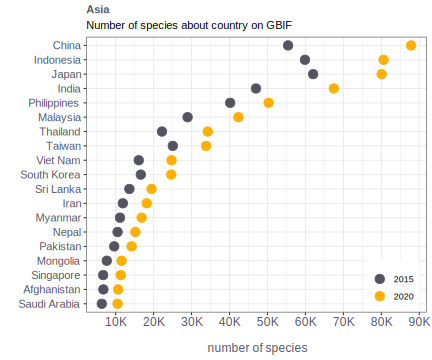
\includegraphics{C:/Users/ftw712/Desktop/gbif_regional_statistics/plots/country dotplots/country_dotplot_species_count_Asia.svg}

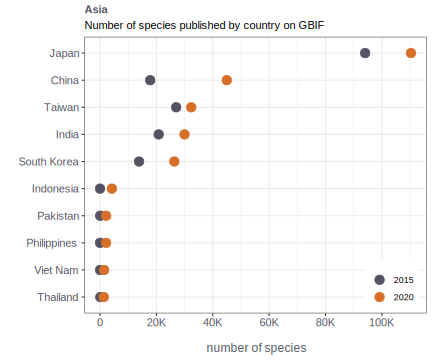
\includegraphics{C:/Users/ftw712/Desktop/gbif_regional_statistics/plots/country dotplots/country_dotplot_species_count_published_Asia.svg}

\includegraphics{C:/Users/ftw712/Desktop/gbif_regional_statistics/plots/country dotplots/country_dotplot_occ_count_Europe.svg}

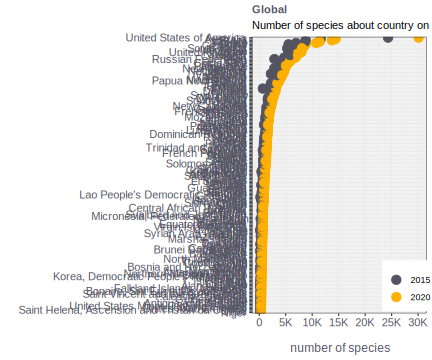
\includegraphics{C:/Users/ftw712/Desktop/gbif_regional_statistics/plots/country dotplots/country_dotplot_species_count_Global.svg}

\hypertarget{stacked-taxanomic-barchart}{%
\subsection{stacked taxanomic
barchart}\label{stacked-taxanomic-barchart}}

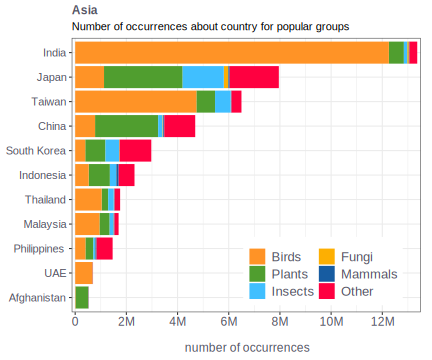
\includegraphics{C:/Users/ftw712/Desktop/gbif_regional_statistics/plots/country stacked barplots/country_stacked_num_of_occ_Asia.svg}

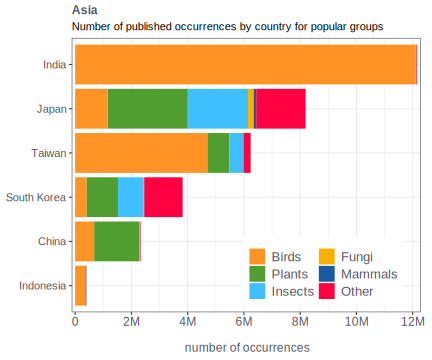
\includegraphics{C:/Users/ftw712/Desktop/gbif_regional_statistics/plots/country stacked barplots/country_stacked_num_of_occ_published_Asia.svg}

\includegraphics{C:/Users/ftw712/Desktop/gbif_regional_statistics/plots/country stacked barplots/country_stacked_num_of_occ_Europe.svg}

\includegraphics{C:/Users/ftw712/Desktop/gbif_regional_statistics/plots/country stacked barplots/country_stacked_num_of_occ_published_Europe.svg}

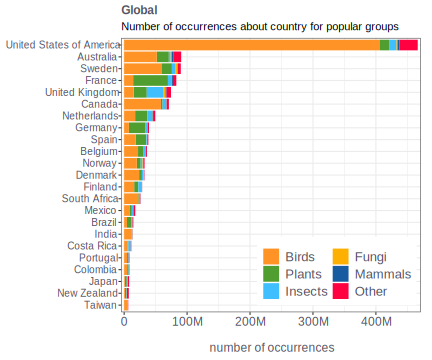
\includegraphics{C:/Users/ftw712/Desktop/gbif_regional_statistics/plots/country stacked barplots/country_stacked_num_of_occ_Global.svg}

\includegraphics{C:/Users/ftw712/Desktop/gbif_regional_statistics/plots/gdp plots/gdp_per_capita_current_us_occ_published_total_full_model_FALSE.svg}

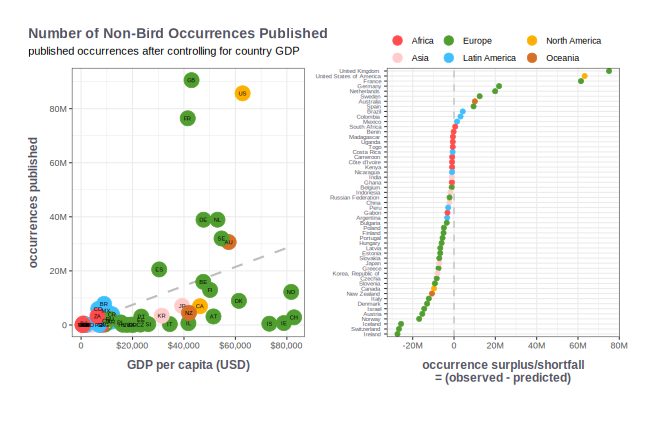
\includegraphics{C:/Users/ftw712/Desktop/gbif_regional_statistics/plots/gdp plots/gdp_per_capita_current_us_num_occ_published_nobirds_full_model_FALSE.svg}

\includegraphics{C:/Users/ftw712/Desktop/gbif_regional_statistics/plots/gdp plots/gdp_per_capita_current_us_num_occ_published_nobirds_full_model_TRUE.svg}

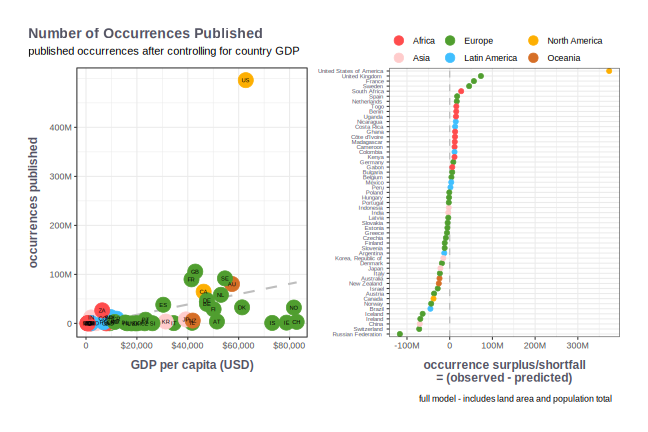
\includegraphics{C:/Users/ftw712/Desktop/gbif_regional_statistics/plots/gdp plots/gdp_per_capita_current_us_occ_published_total_full_model_TRUE.svg}


\end{document}
